% Данный файл распространяетсяя под лицензией CC BY 4.0. Текст лицензии размещён на https://creativecommons.org/licenses/by/4.0/
% (c) Кафедра системного программирования, 2025

\documentclass[a4paper]{article}

\usepackage[a4paper, top=8mm, bottom=8mm, left=8mm, right=8mm]{geometry}

\usepackage[english,russian]{babel}
\usepackage{fontspec}

%\usepackage{fontspec}
\setmainfont{FreeSerif}
\setsansfont{FreeSans}
\setmonofont{FreeMono}

\usepackage[tiny, compact]{titlesec}

\usepackage{titling}
\setlength{\droptitle}{-1cm}
\pretitle{\begin{center}\begin{bfseries}\Large}
\posttitle{\par\end{bfseries}\end{center}}
\preauthor{\begin{center}\normalsize}
\postauthor{\par\end{center}\vspace{-1.8cm}}

\usepackage{hyperref}
\usepackage{bookmark}
\usepackage{csquotes}
% Сюда можно дописывать нужные вам пакеты.
\usepackage{float} 
\usepackage{graphicx}      
\usepackage{caption}       
\usepackage{subcaption}    

\title{Реализация алгоритма Борувки поиска минимального остовного дерева, с использованием библиотеки Spla}

\author{Угарова Полина Павловна}

% Дата много места занимает, её лучше не указывать.
\date{}

\begin{document}

\maketitle

\begin{flushright}
    Группа: \enquote{2025.Б73-мм}

    Кафедра: \emph{кафедра Системного программирования}

    % Степень/звание и должность научника мы лучше вас знаем, их можно не указывать.
    Научный руководитель: \emph{Григорьев Семен Вячеславович}

    % А вот про консультанта укажите официальное место работы, с "ООО" или чем-то таким, и должностью желательно по трудовой, не просто "techlead". Выясните у консультанта.
    Консультант: \emph{Кутуев Владимир Александрович}
    
    Старший инженер-исследователь YADRO
    
    Номер семестра практики: \emph{2}
\end{flushright} 

\section{Введение}
Библиотека \textbf{Spla} \cite{spla_orig, orachev}~--- это библиотека обобщенной разреженной линейной алгебры с открытым исходным кодом и по на графических процессорах (GPGPU). Использование OpenCL (Open Computing Language)~--- открытого стандарта для написания программ, которые используют параллельные вычисления на различных устройствах~--- позволяет Spla работать на GPGPU различных производителей, а также на многоядерных процессорах. Spla использует идеи \textbf{GrpahBLAS} \cite{graphblas} и нацелена на разработку алгоритмов анализа графов.
\section{Постановка задачи}

В рамках проекта по развитию библиотеки Spla уже реализован набор алгоритмов анализа графов, содержащий такие алгоритмы, как обход в ширину (BFS) и PageRank. Однако в библиотеке отсутствует алгоритм для поиска минимального остовного дерева (Minimum Spanning Tree), который и был реализован в рамках данной работы.

Для реализации был выбран \textbf{алгоритм Борувки}, так как он предоставляет естественные возможности для параллельной реализации через операции линейной алгебры, поддерживаемые Spla.

В ходе работы необходимо решить следующие задачи.

\begin{enumerate}
    \item \textbf{Поддержка нового скалярного типа} в Spla~--- пары из номера вершины и веса ребра (\texttt{Pair}), необходимой для работы со взвешенными графами.
    
    \item \textbf{Реализация операций над типом \texttt{Pair}}, образующих полукольцо:
    \begin{itemize}
        \item[$\oplus$] \textbf{сложение/минимум}: выбор пары с минимальным весом. При равенстве весов выбирается пара с меньшим номером вершины.
        \[
        \min((w_1, v_1), (w_2, v_2))
        \]
        \item[$\otimes$] \textbf{умножение/комбинирование}: комбинирование, которое берёт вес из первой пары, а вершину~--- из второй.
        \[
        (w_1, v_1) \otimes (w_2, v_2) = (w_1, v_2)
        \]
    \end{itemize}
    
    \item \textbf{Реализация алгоритма Борувки} с использованием операции умножения разреженной матрицы на вектор (\texttt{mxv}) на основе введённого полукольца.
    
    \item \textbf{Интеграция реализованного алгоритма} в экосистему SPLA с поддержкой GPU-ускорения через OpenCL.
    
    \item \textbf{Запуск} алгоритма на тестовых графах, включая замер производительности.
\end{enumerate}

Результаты работы необходимы для расширения функциональности библиотеки Spla в области графовых алгоритмов. Для конечных пользователей продукта это полезно возможностью эффективного построения минимального остовного леса на GPU. 

\section{Описание предлагаемого решения}
Для представления взвешенных рёбер был введён тип \texttt{Pair}, содержащий вес ребра и номер вершины. Для данного типа были реализованы операции минимума и комбинирования, образующие полукольцо combMin.

\[ \oplus : \min((w_1, v_1), (w_2, v_2)) \]
\[\otimes : (w_1, v_1) \otimes (w_2, v_2) = (w_1, v_2)\]
Использование данного полукольца позволяет выразить поиск минимальных исходящих рёбер через операцию умножения разреженной матрицы на вектор (mxv).

Основные этапы алгоритма.
\begin{enumerate}
    \item Для каждой вершины определяется минимальное инцидентное ребро, ведущее в другую компоненту связности.
    \item Для каждой компоненты связности среди найденных рёбер выбирается одно минимальное исходящее ребро.
    \item Выбранные рёбра добавляются в минимальное остовное дерево.
    \item Выполняется объединение компонент связности, соединённых выбранными рёбрами.
    \item Процесс повторяется до тех пор, пока не останется одна компонента связности. Так как предполагается, что мы работаем только со связанными графами.
\end{enumerate}

Интеграция с существующей кодовой базой Spla потребовала:
\begin{itemize}
    \item добавления нового типа в систему типов библиотеки;
    \item регистрации новых операций в CPU и OpenCL бэкендах;
    \item модификации генератора OpenCL-кода для поддержки пользовательских типов.
\end{itemize}

\section{Эксперименты}
\subsection{Цель экспериментов}

Экспериментальные исследования проводились с целью оценки производительности разработанного алгоритма и анализа факторов, ограничивающих его эффективность. Для этого были поставлены следующие задачи:

\begin{enumerate}
\item сравнить время выполнения реализации на основе Spla с реализацией библиотеки LAGraph на платформе RISC-V;
\item выполнить анализ временных затрат отдельных этапов алгоритма для выявления наиболее ресурсоёмких операций.
\end{enumerate}

Корректность реализованного алгоритма проверялась отдельно с использованием модульных тестов и набора тестовых графов.
\subsection{Среда проведения экспериментов}
Измерения производительности проводились с использованием библиотеки \textbf{graph-bench}~\cite{graphbench}. Для каждого тестового графа выполнялось пять запусков алгоритма, после чего вычислялось среднее арифметическое времени выполнения.

Эксперименты проводились на двух вычислительных платформах.

Первая платформа представляла собой систему на базе архитектуры RISC-V и использовалась для сравнения с библиотекой LAGraph. В качестве OpenCL-устройств применялись GPU PowerVR B-Series, GPU AMD CAICOS, а также многоядерный процессор SpacemiT X60 через реализацию PoCL.

Вторая платформа представляла собой ноутбук с интегрированной графикой Intel UHD Graphics и использовалась для анализа временных затрат отдельных этапов алгоритма. Ноутбук был оснащён процессором Intel Core i3-10110U (2 ядра, 4 потока, 2.10 ГГц) и интегрированным графическим ускорителем Intel UHD Graphics.
\subsection{Оценка производительности с LAGraph}
На рис.~\ref{fig:comparison} представлено cравнения времени выполнения алгоритма на разных OpenCL платформах на RISC-V и с LAGraph реализацией.

\begin{figure}[H]
    \centering
    
    \begin{subfigure}{0.48\textwidth}
        \centering
        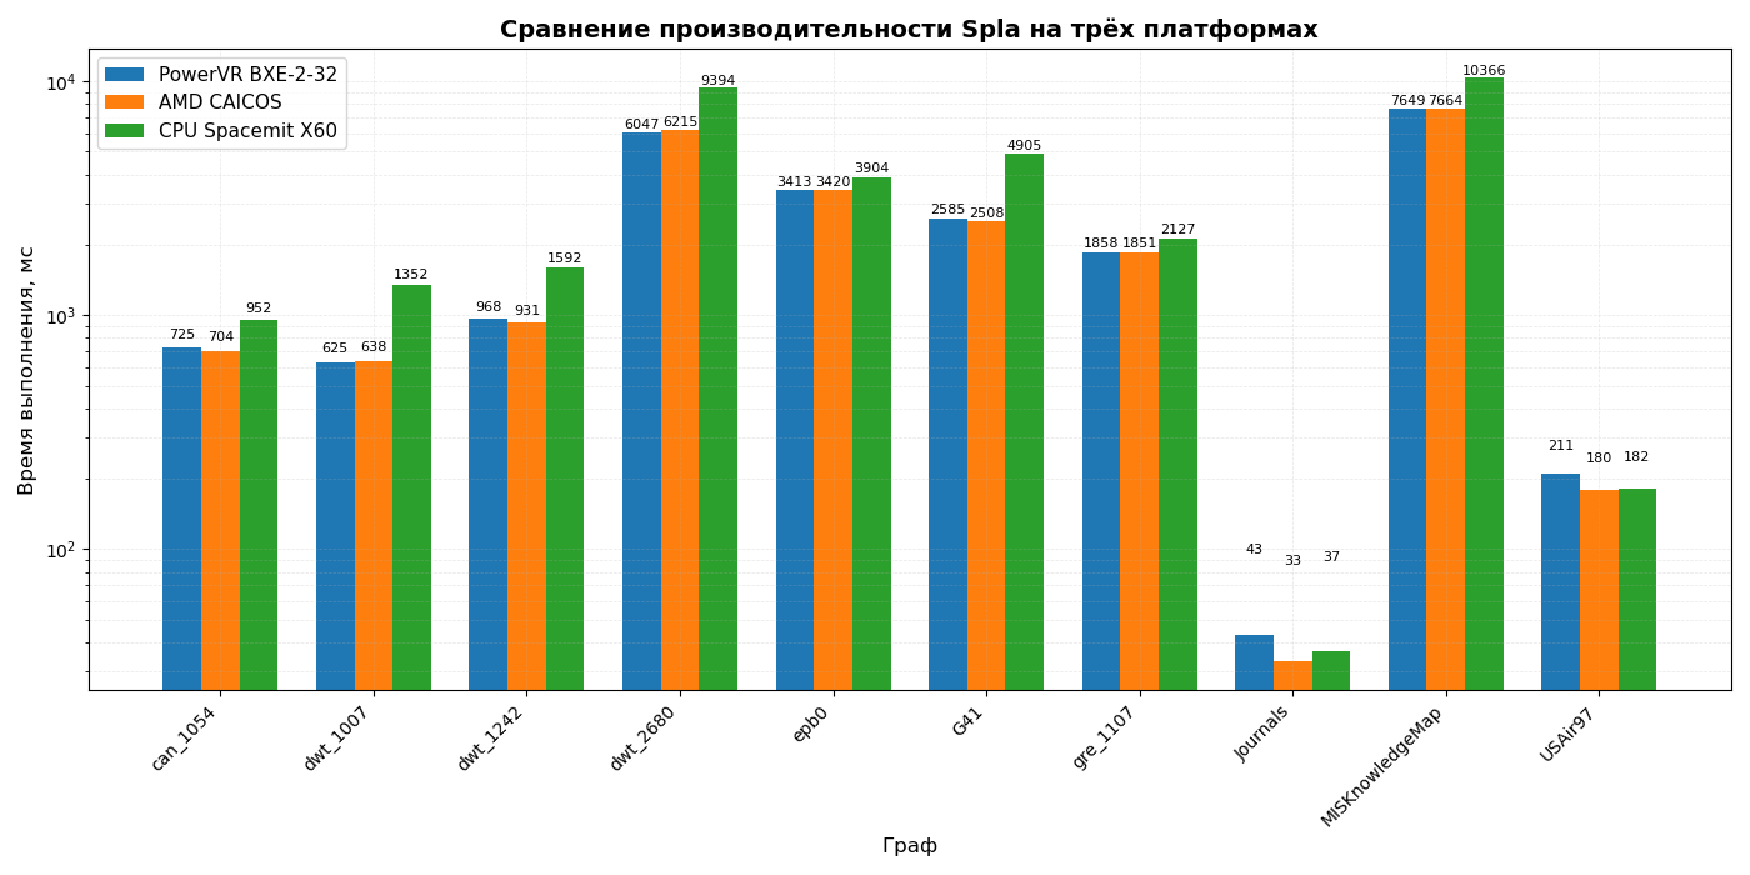
\includegraphics[width=\textwidth]{figures/Figure_1.pdf}
        \caption{Время выполнения алгоритма на различных OpenCL-платформах}
        \label{fig:gpu-comp}
    \end{subfigure}
    \hfill
    \begin{subfigure}{0.48\textwidth}
        \centering
        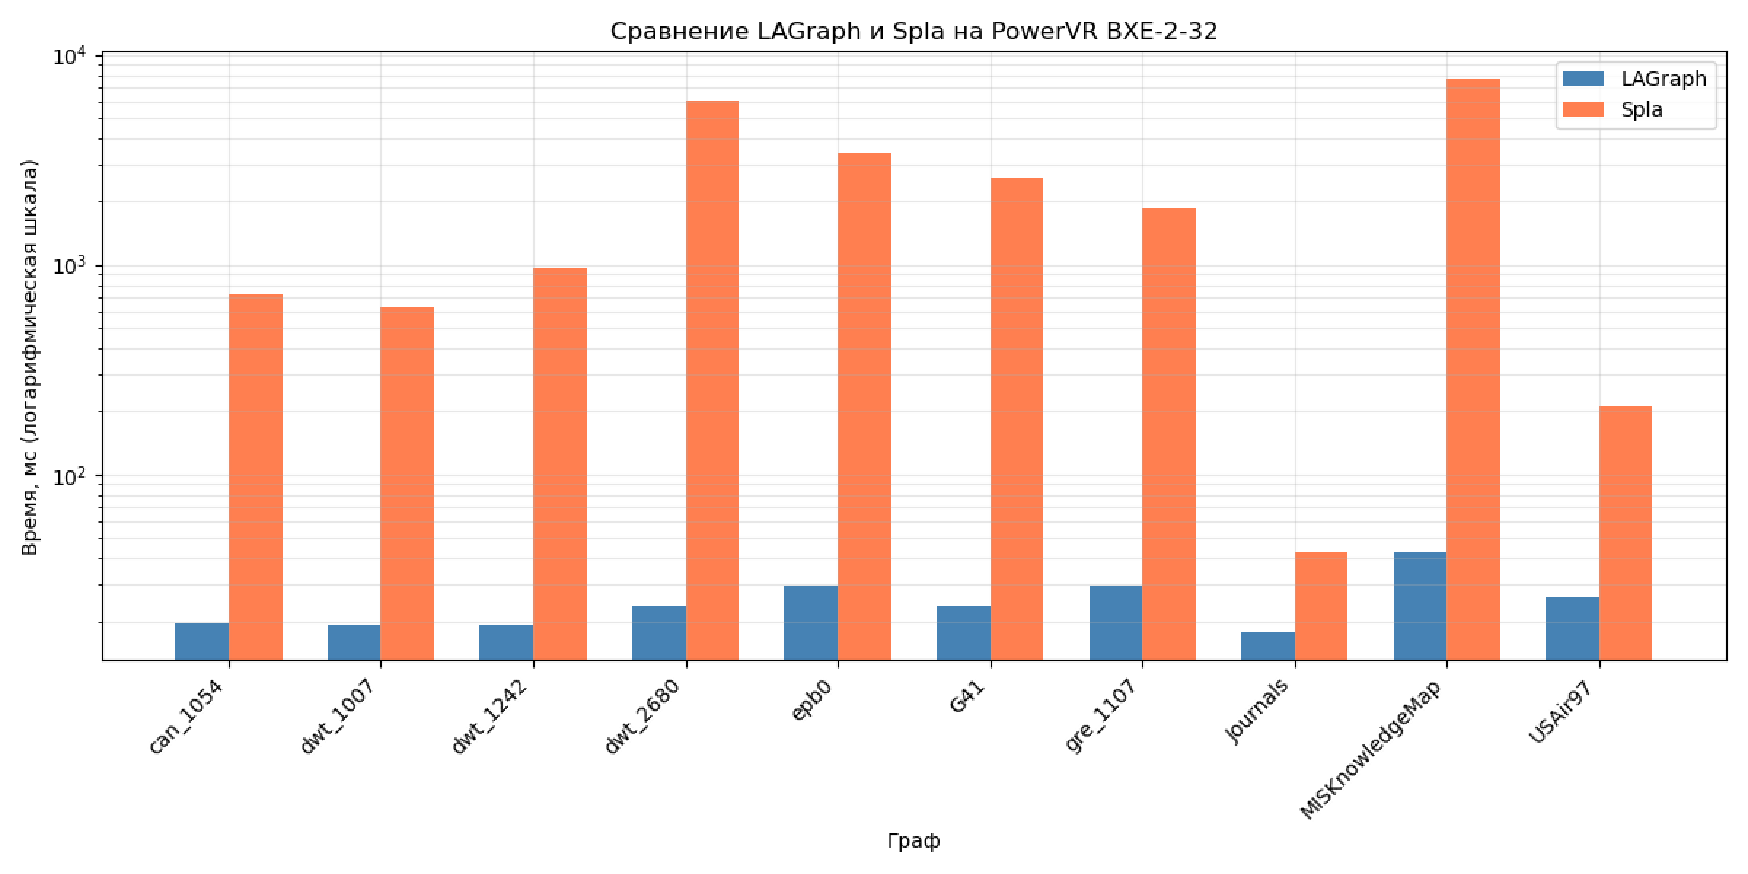
\includegraphics[width=\textwidth]{figures/Figure_2.pdf}
        \caption{Сравнение времени выполнения реализации Spla и LAGraph}
        \label{fig:lagraph-comp}
    \end{subfigure}

    \caption{Сравнение производительности разработанного алгоритма}
    \label{fig:comparison}
\end{figure}


Как видно из рис.~\ref{fig:gpu-comp}, реализация на основе Spla сохраняет переносимость между различными OpenCL-платформами. Согласно рис.~\ref{fig:lagraph-comp}, время выполнения существенно превышает показатели LAGraph: наблюдаемое отставание составляет от 30 до 260 раз в зависимости от используемого графа и вычислительной платформы.

Данный результат свидетельствует о том, что производительность разработанного алгоритма в значительной степени определяется эффективностью базовых примитивов библиотеки Spla.

\subsection{Анализ временных затрат отдельных этапов алгоритма}

Для определения причин наблюдаемого отставания был выполнен анализ времени выполнения отдельных этапов алгоритма. Результаты представлены на рис.~\ref{fig:steps}.

\begin{figure}[H]
\centering
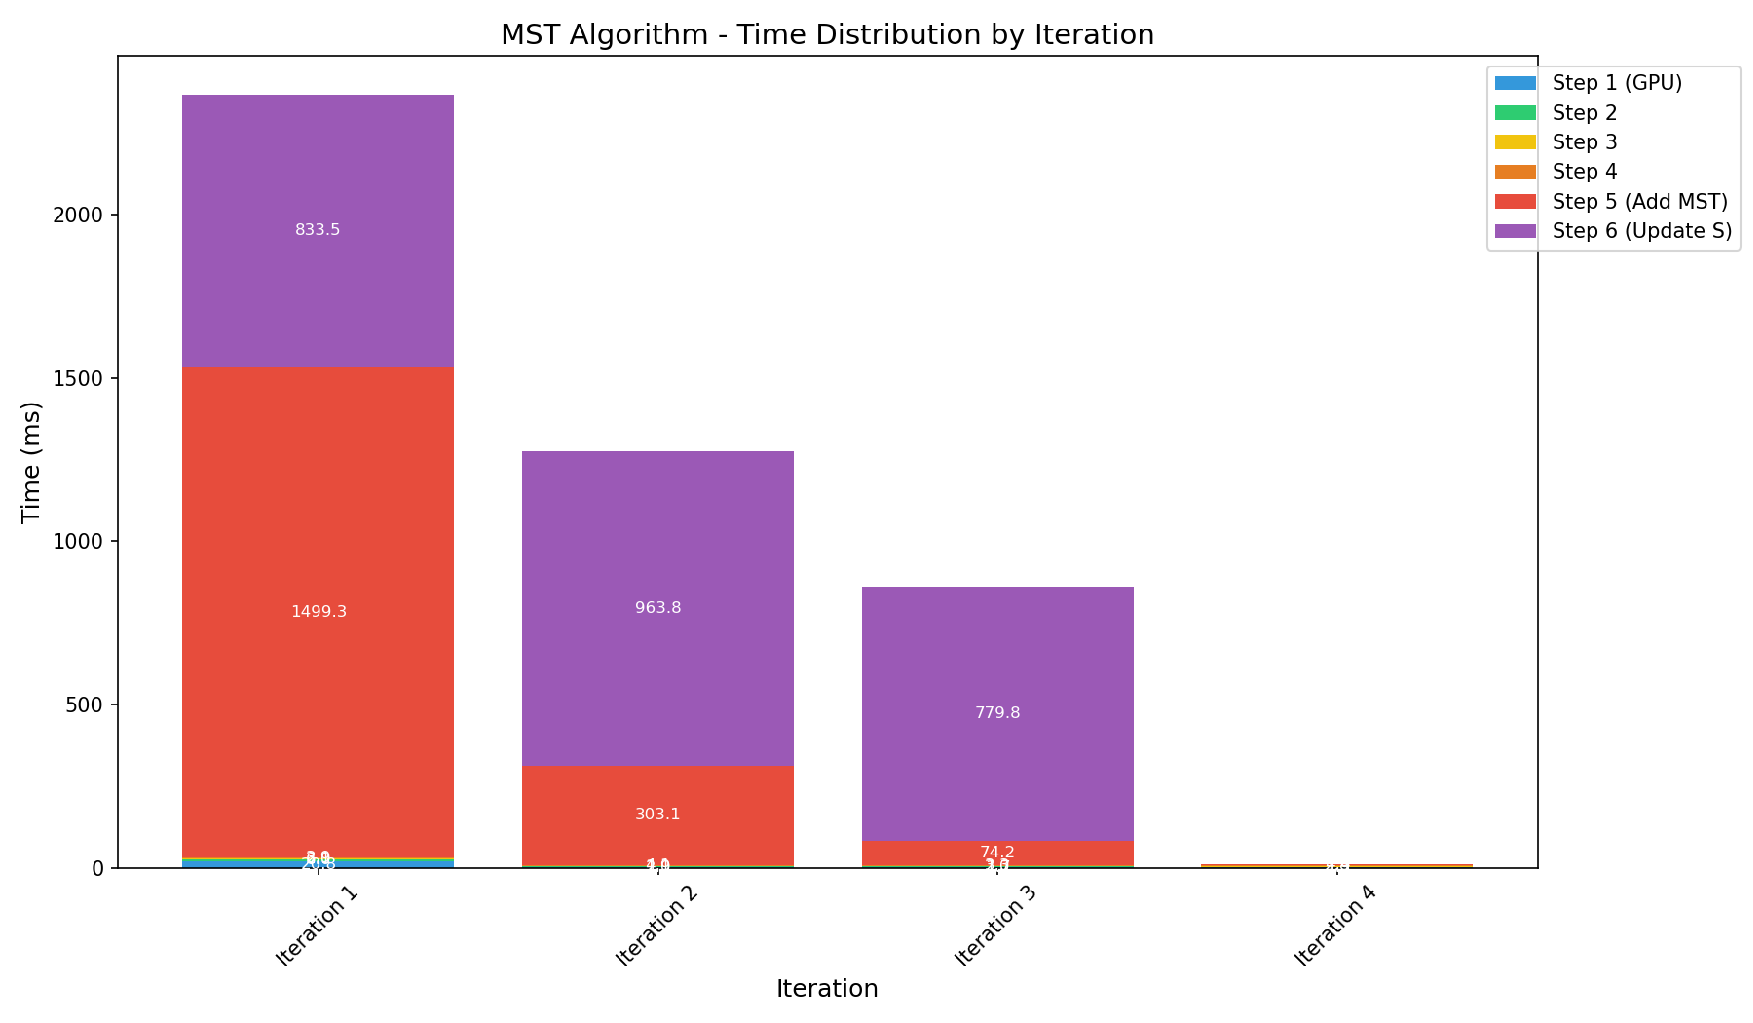
\includegraphics[width=0.6\textwidth]{figures/image.pdf}
\caption{Временные затраты отдельных этапов алгоритма}
\label{fig:steps}
\end{figure}

Как видно из рис.~\ref{fig:steps}, наибольший вклад вносят этапы добавления рёбер в минимальное остовное дерево и обновления компонент связности. На их выполнение приходится более 97\% общего времени работы (4448 мс из 4571 мс).

Причиной этого является отсутствие в Spla GPU-реализаций следующих операций:

\begin{itemize}
\item параллельного добавления рёбер в минимальный остовный лес;
\item параллельной фильтрации внутрикомпонентных рёбер;
\item обновления информации о принадлежности вершин компонентам связности.
\end{itemize}

Указанные операции выполняются последовательно на центральном процессоре и повторяются на каждой итерации алгоритма. В результате преимущества GPU-ускорения, достигаемые на ранних этапах вычислений, существенно снижаются.

Таким образом, реализация перечисленных операций на GPU представляет собой основное направление дальнейшей оптимизации разработанного решения.
\subsection{Апробация}

Результаты работы --- Pull Request в репозиторий Spla.
\begin{itemize}
    \item \textbf{Pull Request:} \url{https://github.com/SparseLinearAlgebra/spla/pull/241}
\end{itemize}
\section{Заключение}

В ходе выполнения работы получены следующие результаты.

\begin{enumerate}
    \item \textbf{Новый тип данных:} в библиотеку Spla добавлен скалярный тип \texttt{Pair} (вес ребра + номер вершины), необходимый для работы со взвешенными графами.
    
    \item \textbf{Операции полукольца:} реализованы операции $\oplus$ (выбор пары с минимальным весом) и $\otimes$ (комбинирование), образующие полукольцо \texttt{combMin}, позволяющее выразить алгоритм Борувки через умножение матрицы на вектор.
    
    \item \textbf{Алгоритм Борувки:} реализован алгоритм построения минимального остовного дерева с использованием примитивов Spla и GPU-ускорением через OpenCL.
    
    \item \textbf{Тестирование:} проведена проверка корректной работы алгоритма на тестовых графах, написаны тесты на операции пары.
    
    \item \textbf{Сравнительный анализ:} произведено сравнение производительности с библиотекой LAGraph на платформе RISC-V, выявлено отставание в 30–260 раз, обусловленное недостаточной оптимизацией примитивов Spla.
\end{enumerate}

Решение не является финальным и открывает направления для дальнейшей работы:
\begin{itemize}
    \item реализация GPU-функций для шагов 5 и 6 алгоритма (добавление рёбер и фильтрация компонент);
    \item оптимизация примитивов SPLA для сокращения отставания от LAGraph.
\end{itemize}
\begin{thebibliography}{99}
\bibitem{spla_orig} Исходный код библиотеки Spla [Электронный ресурс]. URL: https://github.com/SparseLinearAlgebra/spla
\bibitem{orachev} Орачев Е. Generalized sparse linear algebra library with vendor-agnostic GPUs acceleration. URL: https://dspace.spbu.ru/items/2aa43d43-60f5-465d-981d-a8078c69297c
\bibitem{graphblas} Buluç A. et al. Design of the GraphBLAS API for C // 2017 IEEE IPDPSW. — С. 643-652.
\bibitem{graphbench} Исходный код библиотеки graph-bench. URL: https://github.com/EgorOrachyov/graph-bench
\bibitem{lagraph} Исходный код библиотеки LAGraph. URL: https://github.com/GraphBLAS/LAGraph
\end{thebibliography}
\end{document}
